\documentclass[letterpaper, 11pt]{article}
\usepackage {graphicx}
\usepackage{multicol}
\usepackage{hyperref}
\usepackage{geometry}
\geometry{margin=3cm}
\title{	

Genome Wide Association Study using Espresso Methods
}

\author{ Janis Waser}
\begin{document}
\maketitle




\section{Goal}
\label{sec:goal}
Genome wide association studies  (GWAS) are increasingly reliable and thus able to explain biological phenomena. A polygenic risk score is easily computable, but only gives limited insight to the inner mechanisms which are involved. Analyzing all possible combinations by brute-force for large data sets is not feasible and we must find methods which circumvent this complexity and still produce reliable results.

We are using minimal cover algorithms (namely Espresso) to find a small selections of single nucleotide polymorphisms (SNPs) in a causal relationship for a given binary phenotype.  With these selections, we would like to explain the phenotypes.  Further, we investigate the genome-wide spanning relations between SNPs and potential groupings of the phenotype such as different subtypes of a disease. 


\tableofcontents
\newpage
\section {Quality control}
We want to emphasize the importance of quality control (QC) for this approach as it relies heavily on the assumption that the data has no inconsistencies. 

Our data stems from a GWAS/PRS tutorial and the corresponding Git directory which we also use for quality control \cite{tutorial}. It has 109 subjects and 1'073'226 SNPs after the aforementioned QC.  \\



For the selection of approaches the number of permitted unknowns is crucial, which is set to 2\% per individual and SNP. In the scope this means that there might still exist above 20'000 unknowns per individual. 
\section{Espresso}
Espresso is a tool that performs 2-level logic minimisation. It uses heuristics to find a satisfying minimal cover. It takes a logic table as input and outputs a minimized circuit.  The output is not guaranteed to be optimal. \\

"-" can used as don't cares. It is possible to specify special input types such as  \emph{.type fr} to indicate that not in case of an underspecified truth tables the underspecified cases are treated as don't cares. 


\section{Translation of genetic data into binary}
\label{sec:encode}
Most genetic data is stored in two pairwise inherited strings this is true particular for human autosomal genes. The manifestation can be made up from one of the four nucleobases (A/C/G/T) or an indentation of any length or a deletion (non-existence). The information for any particular SNP might also be partially missing. For any given position there commonly exist two different manifestations, one is labelled as the no-risk allele and the other allele is referred to as risk allele. There is no consensus for every SNP on what allele should be considered the risk allele, generally the variant with lower sampling rates is considered the risk allele. Two different studies might find different might find different risk alleles but they would still agree on the same manifestation which is in correlation with the disease. \\


We abstract the manifestations to a count of the occurrences of the risk allele. This count we decode into two digits long binary number. To avoid the unnecessary big Hamming distance of 2 between the counts of 2 ($10_2$) and 1 ($01_2$), while the smaller distance between 2 and 0 ($00_2$) would only have a Hamming distance of 1, we encode 2 as $11_2$. For the effect of this choice consider Figure \ref{fig:binary}.\\

Phenotypes for each individual should already exist in an easily binary translatable form.  We focus on binary phenotypes, if this approach shows promising results it is also possible to extend the approach to continuous  data or different potentially related diseases with pleiotropy. 

\section{Evaluation of results}
\label{sec:evaluate}
We use a range of different criteria to approximate the quality of our method. Each criteria has its own advantages and flaws which should always be taken into consideration. No single criteria is sufficient for showing a working method rather does it give an indication.

\begin{enumerate}
\item Previous identification of SNPs by other researchers
\item Out of data prediction accuracy of the phenotype
\item PRS 
\item Products 
\item Literals
\item Time and complexity of the solution\end{enumerate}

We might also discuss potential issues or perks of a specific method which go beyond this list. 

\subsection{Previous identification of SNPs by other researchers}
If there already exists a genetic analysis on the specific phenotype we are researching, we can compare those findings. 
In other cases, it might even be the case that datasets or phenotypes are simulated. Knowing the underlying structure, we expect our results to match the simulations SNPs, if our method works. 
\subsection{Out-of-data accuracy}
We apply  a k-fold process to our data where we select 90\% of the individuals and the rest serves as out-of-sample data. We can then test the individuals not included whether they satisfy the minimal cover or no and determine whether this deviates from their phenotype.  We expect $2p^2-2p+1$ to be the share of correctly guessed by random guessing where $p$ is the probability of having the phenotype of the "disease". In practice, an ever higher limit should be set at  the max of p  or 1-p as simply always guessing the same outcome would reach this accuracy. 

\subsection{PRS}
PRS or polygenic risk score can be easily determined. It is a single value for each SNP indicating the modelled risk of having the disease when having the risk allele. The distribution of the PRSs is likely to be normal with barycentre around 0. PRS can be simply added up to get a risk score. 
\begin{figure} [!h] \centering{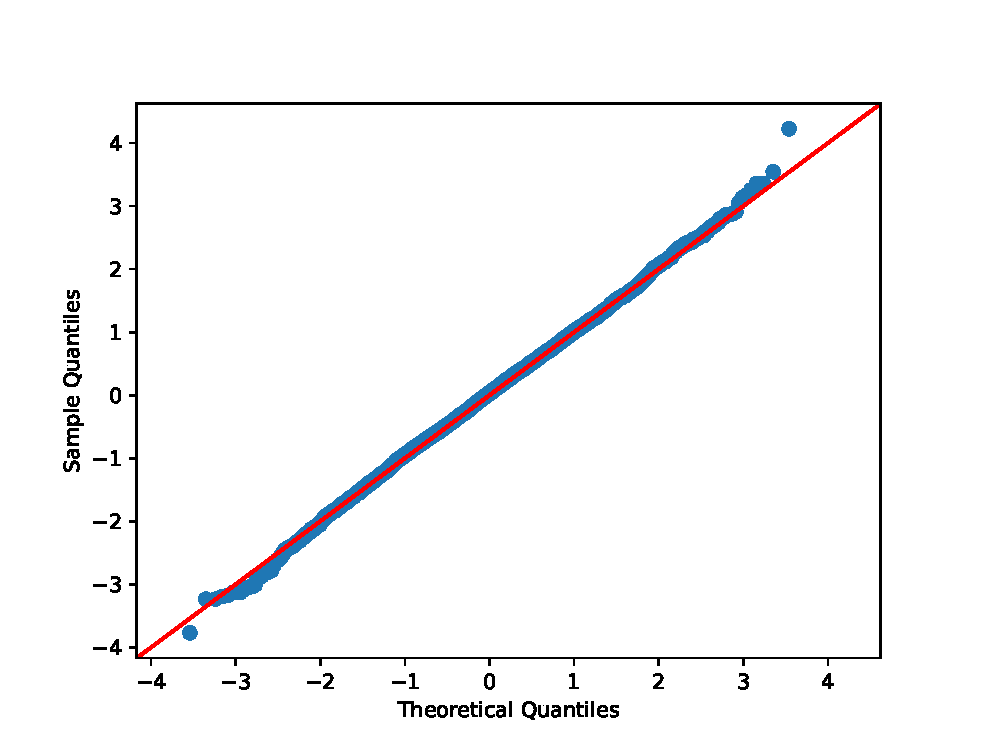
\includegraphics[ trim={0 0 0 0},clip, width=\linewidth]{qq.eps} 
\caption {QQ-plot of combined PRS, clearly distributed normally }\label{fig:qq}
}\end{figure}

It is possible to select a couple of SNPs including their direction (risk/non-risk allele) and calculate a score. If the score is highly positive it indicates predictive power while scores near 0 indicate low predictive power.\\


\begin{figure} [!h] \centering{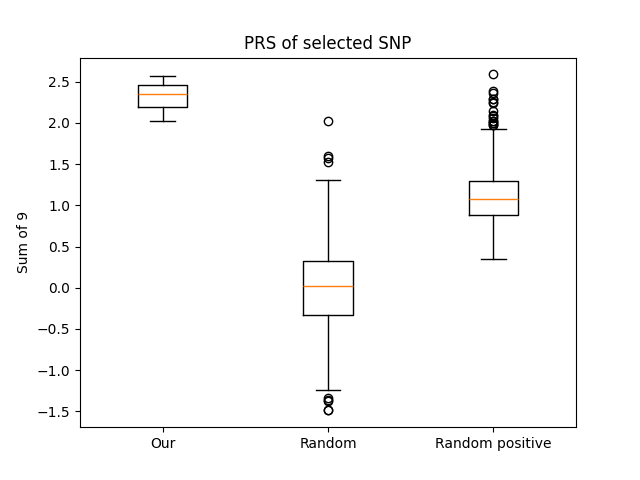
\includegraphics[ trim={0 0 0 0},clip, width=\linewidth]{PRS_selected} 
\caption {Boxplot of PRS of different selections with same size, our selections stem from the pyramid scheme, they deviate significantly from a random selection. }\label{fig:boxplot}
}\end{figure}


For the purpose of analyzing the combined predictive power of SNPs the PRS is not a particularly effective metric as it only states the individual predictive power, which may be obfuscated by balancing out effects. Generally, a high PRS indicates that SNP with high predictive power have been found, but it is not necessary that they are balanced and therefore low scores should a priori not indicate a failure of the method. \\


\subsection{Products}
\subsection{Literals}
\subsection{Time \& Complexity}
\section{ Tried methods}
\subsection{Primitive approaches}
\subsubsection{Entire}
Taking the entire dataset and let it be solved by Espresso, is impossible as the time requirements grow exponentially, as we know the problem is not even in P. 
\subsubsection{Omitting parts of the dataset}
\label{sec:omit}
Taking partial parts of the dataset and never discovering other parts is possible though it is highly doubtful how a good solution should found consistently. For discovering the dataset and experimenting this we did run some experiments. In the context of this experiment when we refer to $n$ we mean the amount of SNPs. 

\begin{enumerate} 
\setcounter{enumi}{1}
\item The out-of-data prediction accuracy is as predicted around the 50\% mark, potentially slightly above for hign $n$. 
\setcounter{enumi}{3}
\item High $n$ yield a smaller product, we explain deviations from this rule by the diverging paths taken in Espresso or in case of different dataset by the difference of possibilities. 
\item Same as for products, just more pronounced as in practice this are higher numbers and therefore more possible outcomes(events). 
\item This analysis is fast and easy to execute for small n, it scales exponentially with n. 
\end{enumerate}


The following table gives an overview of the acquired results with all 109 subjects considered. Each SNP is decoded as two digits, hence the input size is double the amount of selected SNPs. The results are averaged, estimated and depend on the selection of the SNPs and are used as a baseline assumption:

\begin{center}
\begin{tabular}{ c| c| c| c}
 \textbf{Input size (2n)} & \textbf{Products} & \textbf{Literals} & \textbf{Time} \\ \hline
 $<$120& -&-&$<$ 1s\\
 200 & 50 & 3-6&5s\\  
 400 & 40 & 2-4  & 10s \\
 1000& 30&2-3&40s\\
 2000&25&2&8min
\end{tabular}
\end{center}

If there are less than 60 SNP, it is generally not possible to find an assignment as the truth table would be over-specified. \\

A random selection of SNP generally decreases the identified products required for a minimal cover, this trends also affects the literals but is less pronounced. Additionally, it was discovered that missing data is not distributed equally among the data and therefore in sequential analysis even for a relative high n it might not be possible to find a cover due to over-specification. For random selections this constitutes less of a concern as we are guaranteed to have at most 2\% missingness.  
\begin{figure}[h]
\centering{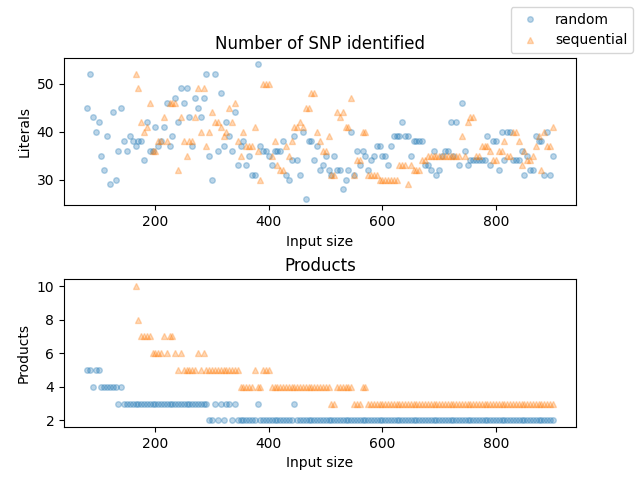
\includegraphics[width=\linewidth]{randseq} \caption {Comparison between random and sequential selection methods }\label{fig:randseq}
}
\end{figure}

The random method will be used exclusively in all future analysis. \\


Different encoding methods also influence the result. The adjusted method is selected going forwards (see \ref{sec:encode})

\begin{figure}[h] \centering{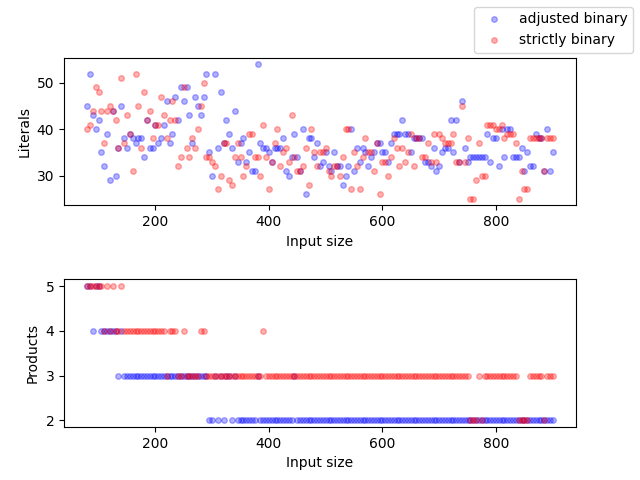
\includegraphics[width=\linewidth, trim={0 0 0 4},clip]{binarycomp} 
\caption {Comparison between different binary encoding methods }\label{fig:binary}
}

\end{figure}

The adjusted method will be used exclusively in all future analysis. 

\subsubsection{Iterative approaches}
We can try to start with some small selection and iteratively build up until the entire data set is included. We start with the smallest possible set such that the truth table is not over-specified and add one SNP, we evaluate this table, find a minimal cover and from the number of literals in the minimal cover, we decide whether this SNP stays in the selection depending on some criteria. Then we do same for every SNP. 

\begin{figure} [!h] \centering{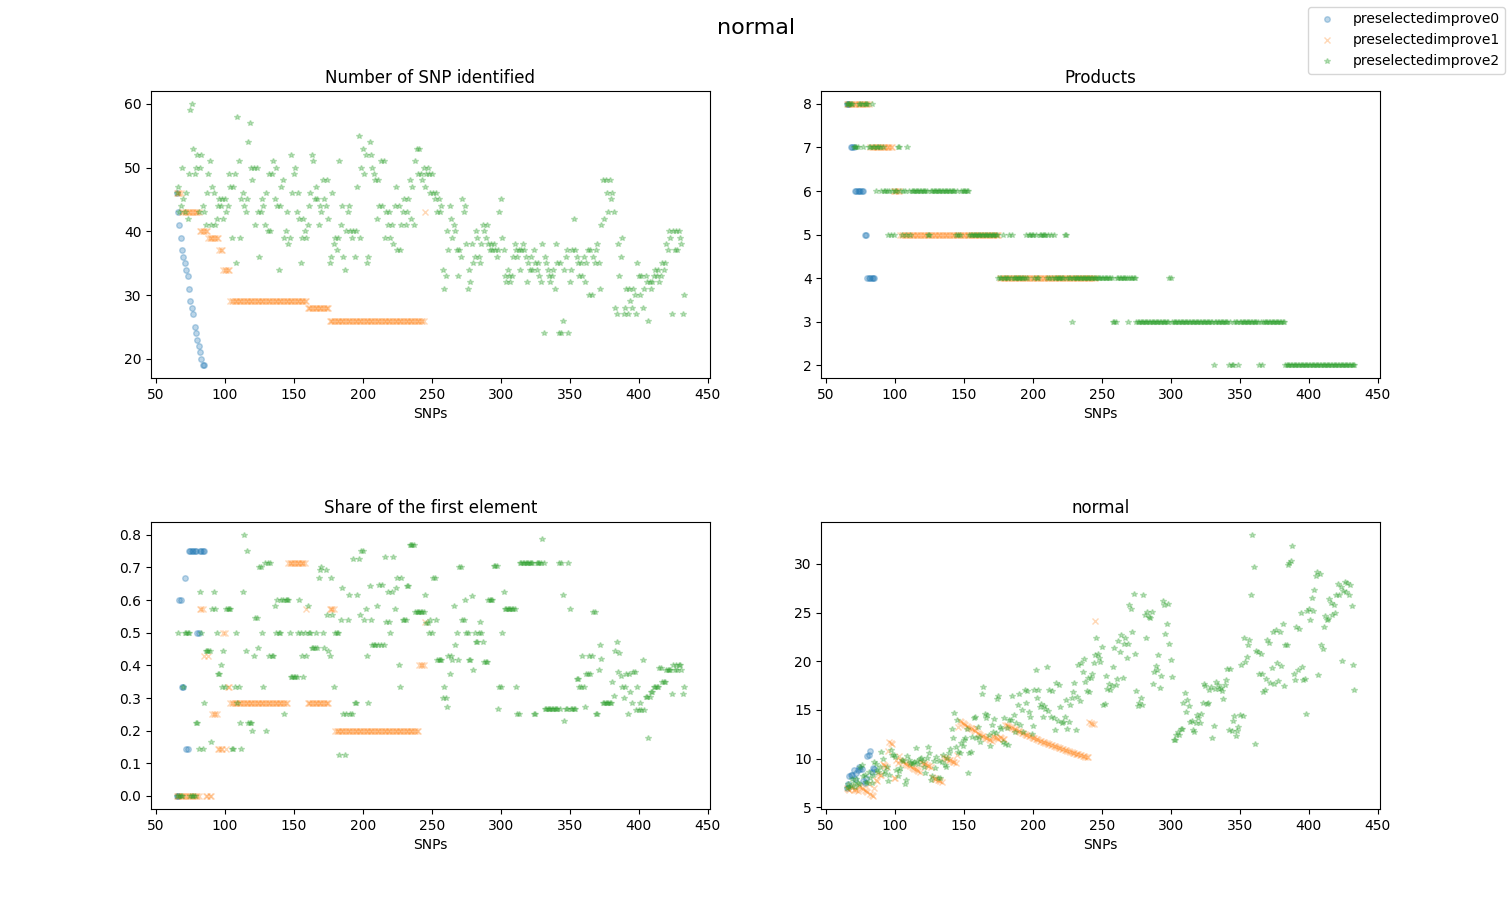
\includegraphics[ trim={70 320 0 0},clip, width=\linewidth]{play_snp} 
\caption {Iterative approaches with SNP indicating the number of selected SNPs, the limit was set on literals. 0: strictly decreasing, 1: monotonically decreasing, 2: no equivalences (increasing or decreasing)}\label{fig:play}
}
\end{figure}

The time it takes to go through the entire dataset is immense and from some point onwards there are likely no gains. This approach does not consider all possible relationships between different SNPs, in fact in only remarks the ones with a strong PRS anyways or the starting set, making this approach not equilibrated. 



\subsection{Pyramid scheme}
In the pyramid scheme, the algorithm runs sequentially  through the entire dataset by separating all SNPs into groups of size $k$, finding a minimal cover for every group. All the SNPs making part of a found minimal cover are then subsequently taken to the next level. This is repeated until in one level  all the identified SNPs from the previous level are less than k SNPs, from where a minimal cover for the entire universe of less than k SNPs can be found. \\

The selection of the group can be done in many ways, we decided to analyze the random selection approach as well as sequential, which should correspond to the sequences in the DNA as already enounced in Chapter \ref{sec:omit}, and clearly preferable as we can see in Figure \ref{fig:randseq}.


\subsection{Phenotype shuffling}
We shuffle the phenotypes of all the individuals, this is achieved through random selection of k persons which have phenotype 2 respectively 1. 
This altered dataset can be run to test different methods. When this is done we expect the resulting minimal cover to be random, meaning that the method we compare to where structure exist should need less literals or products as there is an underlying structure dictating the outcome, where this is obviously not true for shuffled phenotypes. We can also control with the frequencies of the selected SNPs with shuffled phenotypes whether there exists an overlap with the SNPs of our normal method. \\
It was found that not all schemes support phenotype shuffling meaning that for example the grouping scheme relies on the fact that there is some underlying determining for genotypes per phenotype. It therefore might occur that since the involved individuals from one level have an over-specified truth table due to the phenotypes basically being random as the different subgroups of individuals on each level are independent.  \\

\subsection{Grouping scheme}
This method divides the individuals into different equal-sized groups, in each level one group is chosen and the dataset of only those individuals is considered on this level similar to the Pyramid scheme. 

On each level, only a part of the individuals is considered, this means, that the minimal cover is optimized only for those people. On the next level, different individuals get selected, we can assume their phenotype is determined by the same underlying structure, therefore the previous minimal covers should suffice to find a minimal cover. If this is not the case, we have an over-specified truth table, this might be due to there not being an underlying structure or the missing detection of it or due to errors in genotyping. 
\begin{figure} [!h] \centering{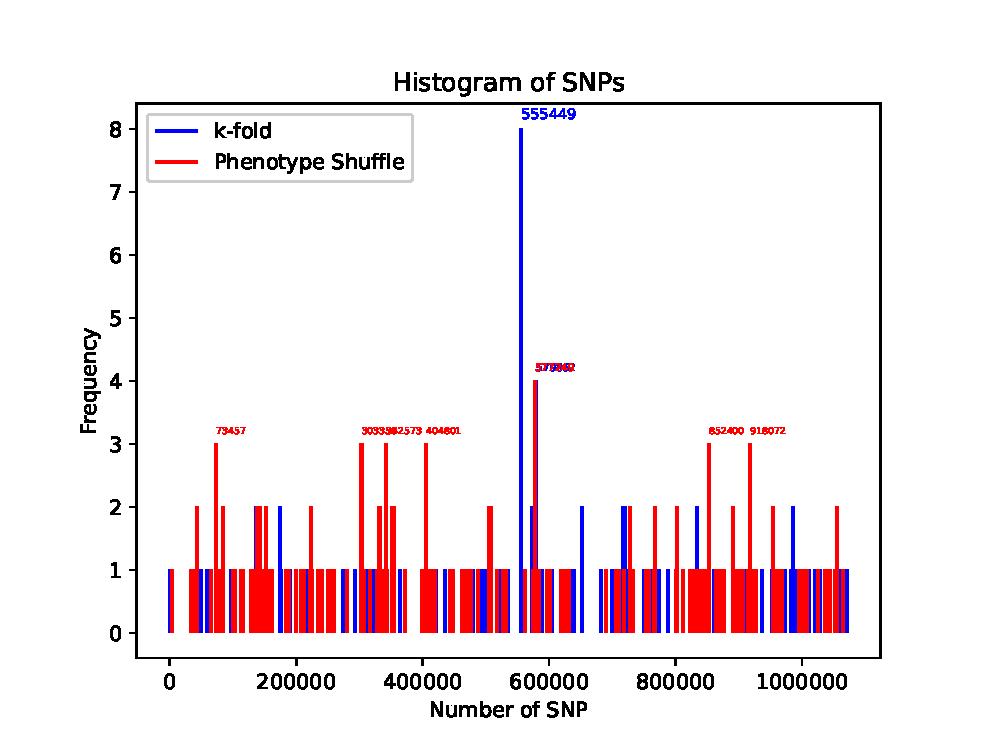
\includegraphics[ trim={0 0 0 0},clip, width=\linewidth]{histall.eps} 
\caption {Histogram of multiple  k-folds using the Pyramid scheme and mutiple phenotype shuffling schemes. The grouping scheme is superimposed on top of the k-fold. No overlap is detected, clear trends with the pyramid scheme are visible, while for shuffled phenotypes no order is apparent.   }\label{fig:play}
}
\end{figure}



\newpage
\begin{thebibliography}{99}
\bibitem{tutorial}
\emph{Marees AT et al. } A tutorial on conducting genome-wide association studies: Quality control and statistical analysis. \url{https://pmc.ncbi.nlm.nih.gov/articles/PMC6001694/}
\bibitem{lipid_data}
\emph{Hajiaghabozorgi, M. } GWAS dataset with simulated binary phenotypes for 1000 Genome Project. March 1, 2023. \url{https://doi.org/10.5281/zenodo.7683384}
\end{thebibliography}
\end{document}